\documentclass{standalone}
% preamble: usepackage, etc.
\begin{document}

\chapter{图匹配推理引擎与符号计算推理的设计和构建}
\section{概况}
在研究设计图匹配推理引擎之前,先介绍一下<<初等数学问题求解关键技术
及系统>>课题。该系统的研究内容主要包括初等数学问题的题意理解和初等
数学问题自动求解两大部分。题意理解就是面向初等数学领域的自然语言处理,
会根据数学领域的自然语言特性,研究针对数学领域的中文分词、词性标注、
命名实体识别、关系抽取、句法分析等自然语言处理基础技术。另一部分,
主要就是根据初等数学问题自然语言理解之后的语义表示,结合问题归约、
认知模型、自动推理、大数据深度学习、图嵌入、符号计算等技术,自动
求解问题并重构类人解答过程。

从上文的介绍中可以看出,图匹配推理引擎主要完成整个系统的第二部分工作
,是自动推理的核心部分。原始的题目文本经过自然语言理解生成的
<实体-关系-实体>语义三元组的json格式数据,该json数据经过统一接口以
图的形式存储在neo4j图数据库中,每一个题目对应一个实例子图,图匹配推
理引擎的输入就是题目的实例子图,输出则是每个实例化规则对应的知识实体。
其主要研究内容包含图匹配推理与计算推理两大部分,共分成四层逻辑架构。
其中图匹配推理研究的内容包括不同推理方式的融合,不同匹配策略,不同的
知识更新策略,以及核心的置换等价问题。计算推理则是依赖于符号计算平台
作为基础支撑,本文最终设计了计算推理与逻辑推理是交互式的推理思想,两种
推理方式相辅相成,让整个推理引擎的功能更加强大,解题的覆盖面也更加广泛。
本章后续的具体小节,将会对图匹配推理引擎与符号计算推理做出详细深入的研究
阐述。
\section{复杂逻辑推理研究}
所谓复杂逻辑推理,顾名思义,即多种推理方式、策略的有机结合而形成的一种
复合的推理方式。相对于单一的推理方式,复合的推理方式不仅能更加准确、
全面的模拟人类的逻辑推理思维过程,还能极大提高系统的解题能力和稳定性。
除此之外,更多的推理方式融合会很大程度上提高了系统的容错率和兼容性。
传统的复杂逻辑推力组合包括基于规则的正向推理与基于规约的逆向推理,
经典分析法与反证法融合推理等。
\subsection{正向推理}
正向推理是从已知事实出发,通过规则驱动,不断产生新的知识实体的一种
推理方式。基于实例化规则的正向推理基本思想是已知事实在规则的驱动下
产生新知识实体,然后新的知识插入到原始事实中去,继续规则驱动,这样
不断知识迭代的一个过程。知识迭代的终止条件就是产生的知识与求解目标
相匹配,表示到达求解目标,求解成功,终止正向推理。如果新产生的知识
与目标知识不匹配,则会将新知识插入到原有的知识库中继续实例化规则匹配,
直到所有实例化规则均不能匹配出发产生新的知识为止。此时表示正向推理
失败,结束正向推理.正向推理的详细推理过程如下图3-1所示:

\subsection{逆向推理}
逆向推理是从目标结论出发,采用分解子目标和规约的基本思想,通过对目标
结论的等价变换、分解成多个子目标的形式,然后从子目标出发,利用分支的
技术,并行规约不同的子目标,一步步递归逆向直到搜寻到已知事实。其推理
流程大致如下图3-2所示:
****************
其算法描述如下:
Begin reverse reasoning
	Search conclusion triples in the questionTriplesSet
		Divide the conclusion triples into multiple sub-conclusion
		New Branch reasoning
			While triple is contained in the map of triple to rule
			Get the rule from the map
				Get the condition triple from the rule 
					If questionTriplesSet contain condition triple
						Recursion and 
					End If 
			End While 
End reasoning  
\subsection{正逆结合}
正逆结合是一种融合了正向推理和逆向推理的复杂逻辑推理方式,这种混合的
推理方式具有兼容性强、推理效率搞、推理方式多样,能较好的模拟人类解题
思维过程等优势。与单一的推理模式不同的是,正逆结合的推理方式,可以
综合已知事实和目标结论,参与推理的信息更加丰富,同时在推理的过程中
两种推理方式也起到互补作用,给各取所长。正逆结合推理分成”先正后逆“、
”先逆后正“两种不同方式。本文最终选择了”先逆后正“的方式进行推理。首先,
逆向推理是系统的入口,逆向推理的主要功能是提高实例化规则选取的效率,
解决正向暴力匹配实例化规则的时间复杂度过高问题。逆推就是通过分解子目标
以及等价规约求解目标,然后递归的去搜寻实例化知识库,递归的终止条件是
已经搜寻到已知事实,并由此构建一棵推理规则树。然后通过逆向推理构建的
规则树回溯出解题路径,将解题路径对应的实例化规则作为正向推理的输入,
开始正向匹配,产生新知识。为了进一步提高解题的效率,正推和逆推中都
使用了分支并行推理技术。下文将会通过举例的方式,详细讲解正逆结合推理
是如何融合正向推理和逆向推理并应用与具体的解题当中。

例3-1,*******************
其推理过程如下图3-3所示:
一般而言,双向推理融合正向推理与逆向推理有三种组合方式:”先正后逆“、
”先逆后正“、”正逆同时“。本文采用是”先逆后正“的推理方式,以下小节将
详细介绍”先逆后正"的双向推理流程和算法。

\subsubsection{先逆后正}
采用“先逆后正”组织结构的双向推理,是将逆向推理作为正向推理的一个重要
补充,逆向推理是构建解题路径的规则树,然后再通过回溯算法输出解题的实
例化规则路径,路径中的每个节点对应就是正向推理的实例化规则,这个路径
作为正向匹配的输入,从而产生每个路径节点对应的新知识。逆向推理相当于
根据已知目标结论出发,有目的性的搜索解题中所使用的实例化规则,这样很
大程度上提高了正向暴力式匹配所带来的时间开销。

“先逆后正”双向推理算法中,逆向推理最基本的思想是分解子目标和等价归约,
然后不断递归这个过程,最终形成归约树,相应逆向推理算法流程为:

*******************

\section{图匹配推理引擎的构建与设计}
图匹配是个经典的图上匹配问题,图匹配问题涉及二分图匹配、最大连通域匹配、
子图匹配等问题。本文设计的图匹配引擎采用的算法思想就是子图匹配算法,又
称子图同构算法。所谓子图同构任务,即给定一个target graph A(m,n),和
一个query graph B(p,q)。其中,m、p是点集,n、q是边集。试图寻找一种
映射关系,使得两个图对应的点label相同,query graph中的边在target 
graph中对应的点之间都存在,且label相同。如下图3-4所示:
*****************
左边图可以同构到右边的上面三角,或者下面三角。
\subsection{引擎基本设计思想}
图匹配推理引擎核心思想是基于图同构的搜索匹配,并寻找一组置换等价的
映射集的复杂逻辑推理引擎。上文已经对图同构进行了阐述,图匹配推理引擎
由图同构的判断器、置换合一的生成器以及知识冲突消解的处理器三大部分
组成。同时也融合了符号计算平台的计算服务、停机等外部接口,为推理引擎
提供计算和停机服务。另外,引擎中还使用了分支并行技术,很好的解决了
多解、分类讨论、等价变幻、知识分解等一些列较为复杂问题,也提升了引擎
并行处理的能力和解题速度。下图3-5是推理引擎的详细结构设计图。
***********************
从图中可以看出,************

\subsection{逻辑架构}
图匹配推理引擎共分为四层逻辑结构,每层结构保持相对独立性。第一层逻辑
结构,图解构层。该层是整个推理的入口,子图的读取就是引擎的输入,对输
入的子图进行解构并转换成推理的数据结构,同时初始化内存各种推理数据流。
下图3-6是推理引擎的第一层逻辑结构图。
*****************
从图中可以看出,*************
第二层逻辑结构,图匹配层。该层是引擎核心部分,具有图同构的判断器和
置换映射集的生成器。第三层逻辑结构,变量置换层。该层依赖于图匹配层,
变量置换的是依据置换映射集生成器生成的置换表,找出若干组变量置换。
同时,该层还调用符号计算平台服务,置换出的变量映射是符号计算接口的
输入参数。第四层逻辑结构,知识更新层。该层是对于变量置换层生成的
新知识进行处理,主要包括知识插入和知识冲突消解两种方式。知识插入
是完成下一轮匹配搜索迭代的前提,知识冲突消解是包括两个部分,知识异常
检测以及知识的冲突检测处理。其中知识异常是指新生成的新知识出现空指针
、不合法、矛盾等情况;知识冲突检测是指新生成知识与已有的知识产生冲突,
需要相应的策略和规则去处理新旧知识,防止出现知识丢失、冗余、重复。

\subsection{Match Engine}
从上文的阐述中,可以看出匹配是整个引擎设计的核心部分。本节会更加详细的
阐述逻辑结构的第二层,图匹配层的整个设计思想和具体结构。下图3-7是图匹配
详细结构图。
**************
从图中可以看出,***********

\subsection{匹配原则}
本引擎匹配最核心的思想,是寻找两组三元组集合是否满足最小子集思想。通过
上文的介绍,题目子图和实例化规则子图都会解构成三元组集合,重新定义三元组
equal的标准:实体类型相同,关系名相同。引擎将实例化规则三元组集合作为最
小子集,在题目三元组集合中搜寻是否覆盖最小子集,为了保证匹配准确度,需要
遵循子集匹配、无方向匹配、组合匹配、自环匹配这四条基本准则。下面将分小节
详细介绍每种匹配原则。其伪代码描述为:
For RuleRelationMap is not Empty
	For QuestionRelationMap is not Empty
		If qRealtionSet contains rRealtionSet
			Select matching strateges according to qRelationSet 
				If rTriple match to multi-qTriples
					Enter into conbinationMatch model
						Refresh the Map of questionEntity to ruleEntity 
						detach fake match conbination
				Continue
				End If
		End If
		Print some error log about match
	End For
End For

****************
\subsubsection{子集匹配}
子集匹配是保证引擎有较好兼容性和通用性的一个重要原则。子集匹配的对象是
三元组中实体类型。子集匹配的定义:给出两组三元组,若它们的实体类型具有
继承关系,可以是直接的父类子类继承,或满足间接继承关系,则两组三元组满足
子集匹配。下面以一个例子进行说明,题目三元组<等差数列-项关系-首项>,规则
三元组<数列-项关系-项>,等差数列直接继承于数列,首项直接继承于项,因此
两个三元组满足子集匹配原则,属于可匹配三元组。
\subsubsection{无方向匹配}
无方向匹配是增加引擎匹配搜索灵活性,增大了匹配搜索的范围。知识图谱中
存储的题目和实例化规则子图都是以有向图形式存储的,因此三元组均是有方
向的。无方向匹配原则是指将三元组匹配进行两次匹配检测,第一次完成正向
就检测,匹配成功退出返回0;匹配失败则将三元组进行逆向匹配检测一次,
匹配成功退出返回0,匹配失败返回-1。例如,题目三元组<反比例函数-区间关系-区间>,
实例化三元组<区间-区间关系-反比例函数>,则需要进行两次匹配检测,满足
无方向匹配原则,属于可匹配三元组。
\subsubsection{组合匹配}
组合匹配是指一个三元组或一组三元组能匹配上两组或两组以上的三元组集合,
这个时候边会出现组合问题。组合匹配形式主要有一对多,多对多的情形。从
形式定义和概念上组合匹配较为容易理解,但是如何正确的处理组合分支、
组合爆炸是个比较疑难的问题。本文对于组合匹配问题采用了多重解决方案,
并在具体题目得以验证和应用。当遇到组合匹配时,基本原则是将组合匹配
转换成单一匹配,然后通过循环的方式去完成组合。组合的情况较为复杂,以下
将通过例子来列举组合发生的几种情况。

例1,实例化三元组<数列-项关系-项>,题目三元组集合{<等差数列-项关系-首项>,
<等比数列-项关系-项>},这是最常见的三元组组合情形,引擎处理的手段是将题目
三元组集合拆成等价于最小实例化三元组的多组,然后依次匹配或采用分支技术并
行匹配。例2,实例化三元组{并集AuB-子表达式关系-集合A,并集AuB-子表达式关系-集合B}
题目三元组{并集MuN-子表达式关系-集合M,并集MuN-子表达式关系-集合N,
并集PuQ-子表达式关系-集合P,并集PuQ-子表达式关系-集合Q},此组合
对应于多对多的一种情形,若按照组合学方案会有6种组合方式,这样会产生
4组多余的组合出来,若四组知识继续插入到知识库,进行下一轮的匹配循环
迭代会继续产生越来越多的知识,最终便会组合爆炸。如何寻找有效组合,排除
假组合,将在下文详细介绍。

对于上文例2的组合情形,引擎会启用三种机制去筛选假组合。方案一:属性标价法。
属性标记法,是通过在关系中添加一个属性字段isGroup来标记三元组是否属性同一组,
同一组的定义是两个或两个以上三元组具有共同的头实体或尾实体。属性标记法通过
属性字段来对相同三元组进行分类处理,先分类再匹配,这种方式可以有效的降低
组合次数,例2中题目三元组四个相同三元组,通过isGroup属性标记分类,化分成
{并集MuN-子表达式关系-集合M,并集MuN-子表达式关系-集合N}和
{并集PuQ-子表达式关系-集合P,并集PuQ-子表达式关系-集合Q}两类,分类完成后将
原有的随机组合6组降成为2组有效组合,筛选掉4组多余组合,大大提升了匹配效率。
\subsubsection{自环匹配}
自环匹配是弥补匹配设计缺陷,匹配的最小单位是三元组,因此匹配子图的限制条件
确保能解构成三元组集合,不能存在离散的孤立节点。为了让推理引擎通用性更高,
引擎对孤立节点情况做了自我完善。当实例化规则子图中出现自环节点时,引擎
会自动检测同类型的题目节点并增加一条自环关系,解构后的三元组集合多出相应
的自环三元组。
\subsection{置换合一}
在谓词逻辑中,推理被定义为从一定的合式公式和合适公式之间通过推理规则,到
产生新的合式公式的过程。最常用到的两种推理方式时假元推理和全称化推理。由
合式公式W1和W1->W2产生合式公式W2的推理过程叫假元推理。再比如,由合式公式
(x)W(x)产生合式公式W(A)的推理过程,其中A是常量符号x是变量符号,叫全称
化推理。全称化推理中的常量符号A替换变量符号x的过程,叫做置换(Substitution)。
表达式置换就是用置换项置换变量的过程。谓词逻辑中的表达式置换在人工智能中
具有非常重要的意义,他体现的是一种演绎的思想。这里有5点应该理解的:
(1)被置换元素是变量,置换元素是项。
(2)置换元素不同于被置换元素,否则置换是无意义的。
(3)在同一次置换中,针对同一变量的置换操作只能进行一次。或者说,同一
表达式中的不同变量同时置换,并没有先后之分。
(4)无元素的置换被成为空置换。
(5)
寻找项对变量的置换是两个表达式一致,叫合一(Unification)。与置换不同的,
合一更多是体现对表达式的抽象和归纳思想。如果一个置换s作用与表达式集{Ei}
中的每个元素,使得E1s=E2s=...Ens,则称表达式集{Ei}是可合一的,此s称为{Ei}
的合一者(Unifier)。
\section{知识更新}
知识更新是当前轮匹配和下一轮匹配迭代的重要衔接。引擎处理知识更新的技术手段,
知识插入、冲突消解、更新回代、自动停机等。知识插入是对实例化规则产生的新知识
插入到原有的题目知识图谱中,是知识更新最基础也是最重要的手段。知识更新流程如
下图3-8所示:
*****************
根据图3-8所示的知识更新流程图的描述,其对应的知识更新算法伪代码解释如下所示:
Knowledge Entities:
	Knowledge exception detach
	If Knowledge is null or illegal,end refresh
	If match successfully:
		Add conclusion triple
		Calculator the sign of refresh type
			select the plan according to the sign
			Insert Knowledge entity or relation into question graph
			Check whether the stop conditions are met
			If the Know
			ledge belong to Equation
				Add the Knowledge into Equation Collector
			End If
	End If
End If
知识更新是正向推理迭代思想至关重要的环节,算法中冲突消解体现在知识合法性检测上。
冲突消解有以下几种情景:
(1)新知识为空或者空字符串
(2)出现恒等式、矛盾式,如“1=1”,“1=-1”
(3)多解,知识冗余
(4)新知识插入时已经存在同类型的知识,类型变元相同或者重复都会造成冲突。
\section{类人解答过程的构建}
类人解题是指一道题目的求解机器和人类求解类似,解答过程是伴随着“因为xxxx
所以xxx”的严密逻辑、计算思维过程。重构类人解过程是指从推理知识库中找到
求解问题相关知识之间的逻辑、计算关系,从而构建一条从已知到结论的完整解题
路径。此模块是依赖于推理模块的逻辑推理和计算推理,在推理的同时构建解答
过程规则树,最终的输出就是对规则树进行回溯,得到类人解答过程,适用范围
是选择题、填空题、解答题。输出的形式是两种,第一种是后端以Log日志的方式;
方式二是知识图谱的形式呈现解答过程子图。	

\subsection{类人解题的前提}
由于重构解题路径中体现的逻辑关系是基于图匹配推理引擎中实例化规则选取
体现的逻辑关系和符号计算推理实现的,因此最后重构的解答过程中包括的
因果逻辑关系的粒度取决于实例化规则和符号计算的粒度。为了保证最后的
解答过程正确且不重复,需要合理选取实例化规则和符号计算的粒度。如果
规则粒度过粗,最后的解答过程会出现遗漏或者跳跃的情况;如果粒度过细,
将会出现解答过程冗余,多了很多可以省略的步骤。例如,实例化规则为求
函数单调区间。推理中使用此规则时,该规则在调用符号计算服务时会省略
一些必须的过程,如:其函数导函数,令导函数为零,求解导函数方程,
结合定义域讨论方程的解,根据定义域讨论单调区间等。如果规则粒度过细,
这些求导的过程都呈现在解答路径中,会让后台Log日志和解答过程子图
显得冗余。同时还会导致推理效率变低,知识库压力增大。所以,保持
一致的、适当的实例化规则粒度,是类人求解的必要前提条件。

还有一点需要注意的是知识实体的显示。图匹配推理引擎的知识实体都是
以三元组(Triple)形式表示,他们是自然语言对应的计算机结构化的
知识描述。而类人解答过程中体现的知识是面向人交互,需要将三元组
转换成自然语言的形式描述出来。在形成解答过程中可能包含一些必要
的属性描述,一般做法是将所有实体(Entity)和关系(Relation)的
父类(这里是AbstractData和AbstractRelation)中添加一个抽象函数,
每一个不同子类下具体实现各自的抽象方法。
\subsection{重构类人解答}
重构类人解答过程一般分为两步:一,在推理过程构建解答过程规则树,
并对树中每个节点编号;二,对规则树进行回溯算法,生成可读过程和
解答过程子图。

\subsubsection{实例化定理编码}

\subsubsection{构建解答过程}
重构的过程是对规则树遍历和回溯的过程,对遍历回溯的结果组成“因为所以”
的逻辑,本质上是先序遍历和回溯算法。当访问一个事实时,如果是已知事实,
直接加上编号作为“因为”部分;否者,加上他对应的编号作为“所以”部分。其
伪代码描述为:
*******************
\begin{table}[h]
	\caption{计算$2m\times 2m$理想导体平板时域感应电流采用的三种存储方式的存储量比较。} 
	\begin{tabular}{|c|c|c|c|} 
		\hline  
		时间步长 & 非压缩存储方式 & 完全压缩存储方式 & 基权函数压缩存储方式 \\
		\hline 
		0.4ns & 5.59 MB & 6.78 MB & 6.78 MB\\  
		\hline  
		0.5ns & 10.17 MB & 5.58 MB & 5.58 MB \\  
		\hline  
		0.6ns & 8.38MB & 4.98 MB & 4.98 MB \\  
		\hline  
	\end{tabular}
	\label{tablea}
\end{table}

如图\ref{picd}所示给出了时间步长选取为0.5ns 时采用三种不同存储方式计算的
平板中心处$x$方向的感应电流值与IDFT 方法计算结果的比较,……。如图\ref{pice}
所示给出了存储方式为基权函数压缩存储方式,时间步长分别取0.4ns、0.5ns、0.6ns
时平板中心处$x$方向的感应电流计算结果,从图中可以看出不同时间步长的计算结果基本相同。

由于时域混合场积分方程是时域电场积分方程与时域磁场积分方程的线性组合,因此时域混合场积分方程时间步进算法的阻抗矩阵特征与时域电场积分方程时间步进算法的阻抗矩阵特征相同。

\begin{figure}[h]
	\subfigure[]{
		\label{picd}
		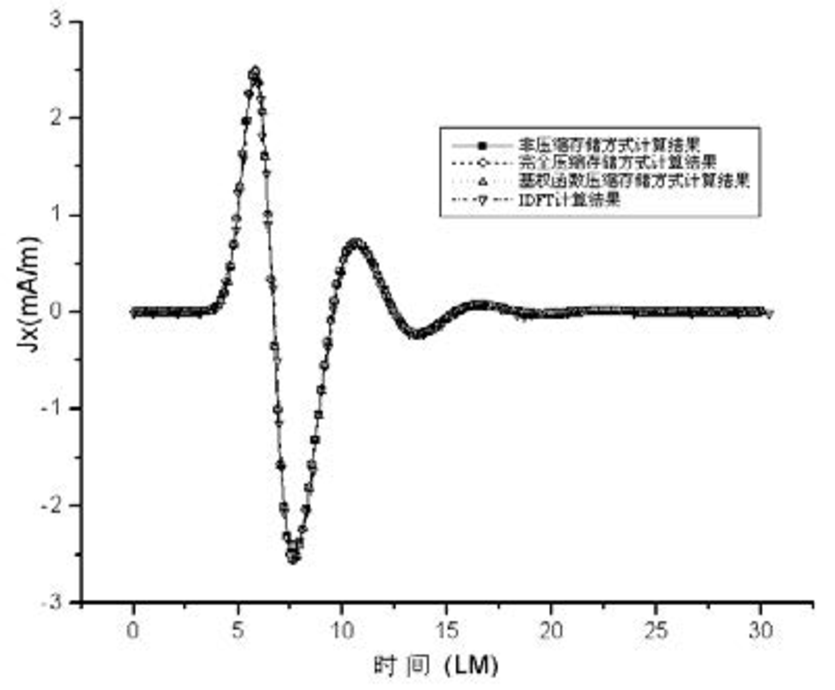
\includegraphics[width=6.77cm]{picd.pdf}}
	\subfigure[]{
		\label{pice}
		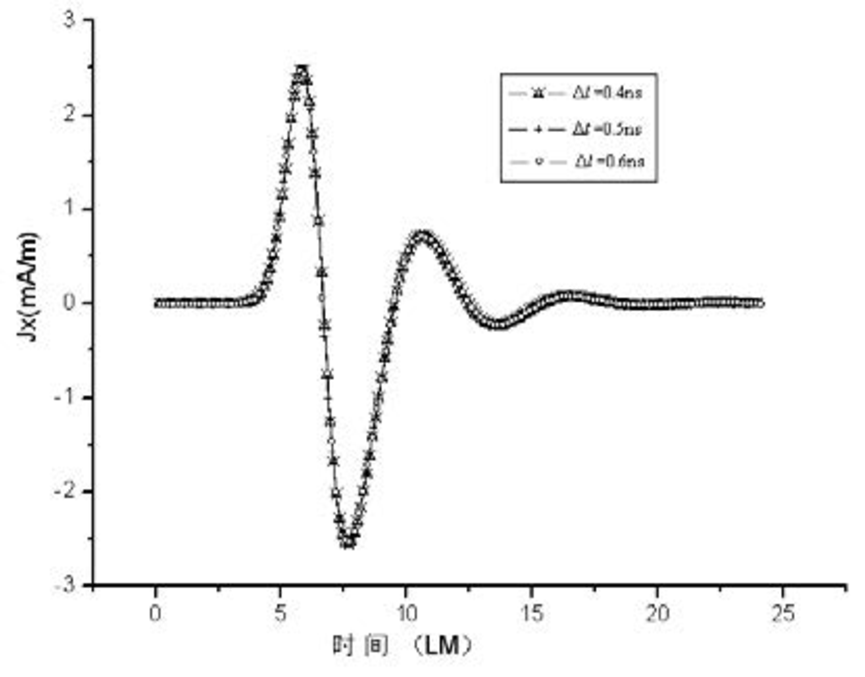
\includegraphics[width=7.04cm]{pice.pdf}}
	\caption{$2m\times 2m$的理想导体平板中心处感应电流$x$分量随时间的变化关系}
	\label{fig2}
\end{figure}


由于时域混合场积分方程是时域电场积分方程与时域磁场积分方程的线性组
合,因此时域混合场积分方程时间步进算法的阻抗矩阵特征与时域电场积分方程
时间步进算法的阻抗矩阵特征相同。
\section{时域积分方程时间步进算法矩阵方程的求解}

\begin{theorem}
	如果时域混合场积分方程是时域电场积分方程与时域磁场积分方程
	的线性组合。
\end{theorem}
\begin{proof}
	由于时域混合场积分方程是时域电场积分方程与时域磁场积分方程的线性组
	合,因此时域混合场积分方程时间步进算法的阻抗矩阵特征与时域电场积分方程
	时间步进算法的阻抗矩阵特征相同。
\end{proof}
\begin{corollary}
	时域积分方程方法的研究近几年发展迅速,在本文研究工作的基础上,仍有以下方向值得进一步研究。
\end{corollary}
\begin{lemma}
	因此时域混合场积分方程时间步进算法的阻抗矩阵特征与时域电场积分方程
	时间步进算法的阻抗矩阵特征相同。
\end{lemma}

\section{本章小结}
本章首先研究了时域积分方程时间步进算法的阻抗元素精确计算技术,分别
采用DUFFY 变换法与卷积积分精度计算法计算时域阻抗元素,通过算例验证了计
算方法的高精度。

\end{document}